% ============================================================
% ============================================================
% NACA0012 -- ICE ACCRETION
% ============================================================
% ============================================================

\section[Ice]{\textbf{Ice Accretion}}


% ============================================================
% ============================================================
% NACA0012 -- Ice Mass Grid Convergence
% ============================================================
% ============================================================

\begin{frame}{\small NACA0012 -- Ice Mass Grid Convergence}
\scriptsize

\begin{columns}[T,onlytextwidth]

\begin{column}{0.50\textwidth}
    \centering
    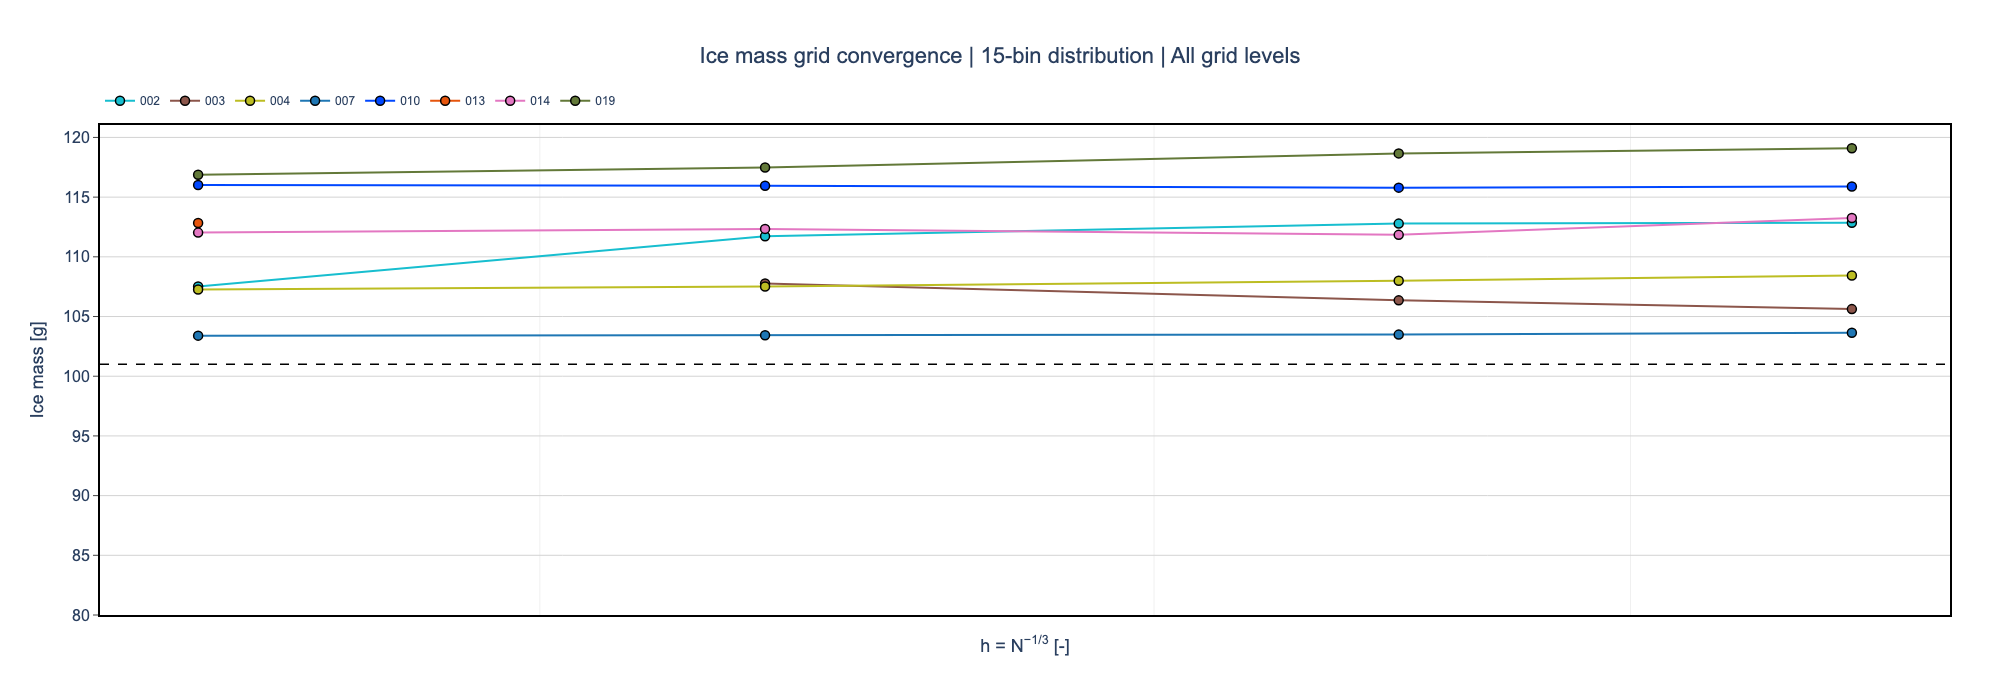
\includegraphics[width=\textwidth]{FIGURES/ICE_ACCRETION/tc_naca0012_ae3932_ice_mass_vs_n_unspecified_bins15_all_grid_levels.png}

    \vspace{0.05cm}

    {\scriptsize\textbf{AE3932}}
\end{column}

\begin{column}{0.50\textwidth}
    \centering
    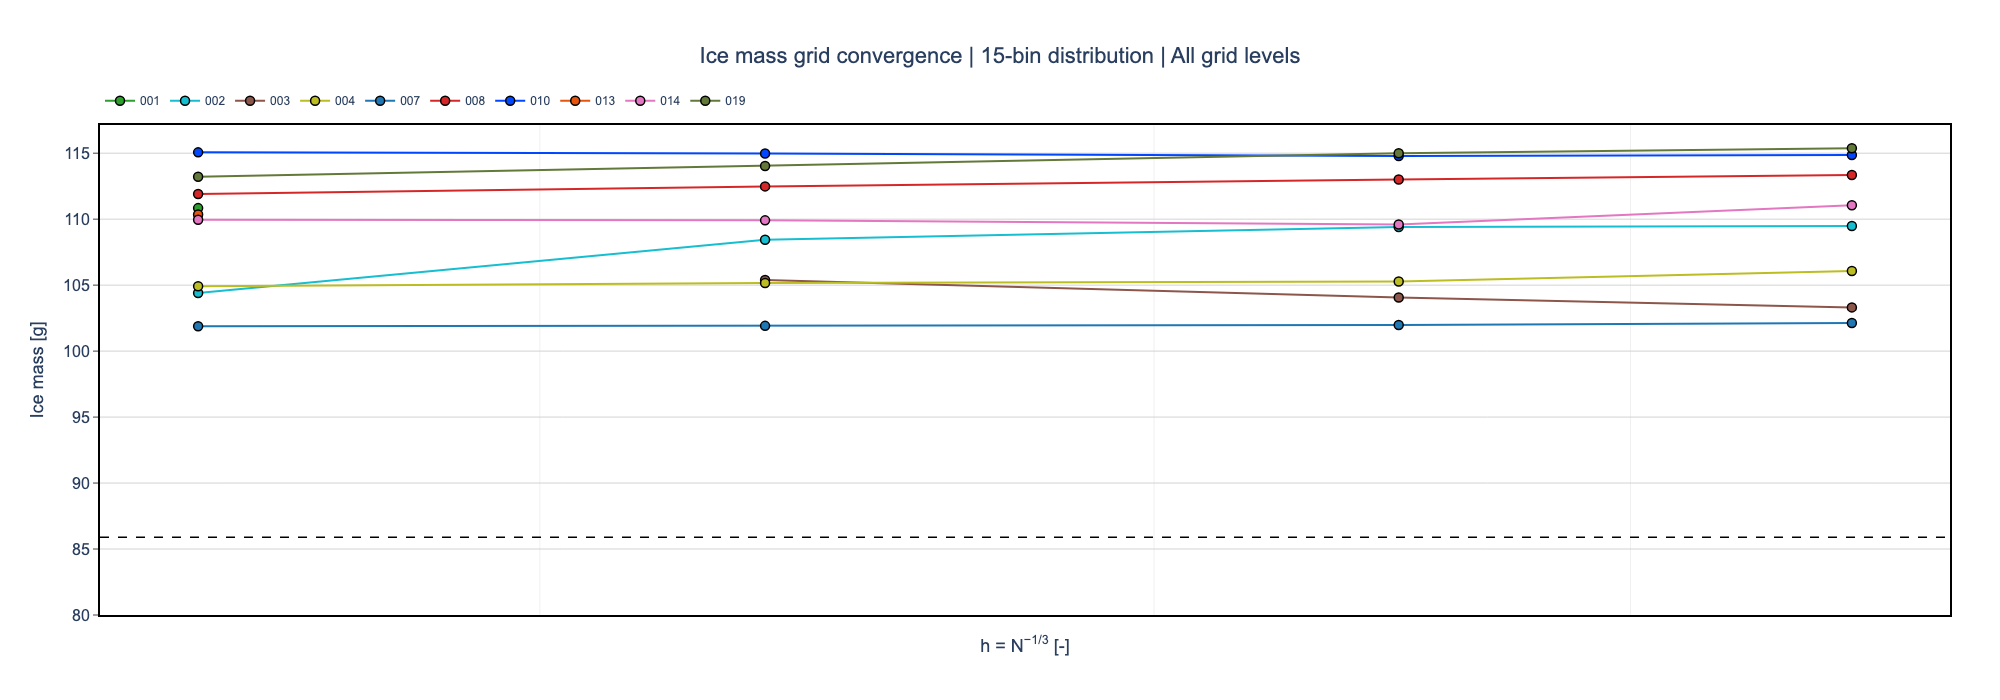
\includegraphics[width=\textwidth]{FIGURES/ICE_ACCRETION/tc_naca0012_ae3933_ice_mass_vs_n_unspecified_bins15_all_grid_levels.png}

    \vspace{0.05cm}

    {\scriptsize\textbf{AE3933}}
\end{column}

\end{columns}

\vspace{0.15cm}

\begin{block}{\scriptsize Assessment}
\begin{itemize}
    \item Most submissions exhibit limited ice-mass sensitivity to spatial grid refinement for the 15-bin distribution.
    \item An isolated submission exhibits substantially stronger grid sensitivity than the main participant cluster.
    \item Code-to-code differences remain visible on the finest grid and cannot be attributed solely to spatial resolution.
    \item A systematic difference between AE3932 and AE3933 begins to emerge in the predicted ice mass.
\end{itemize}
\end{block}

\end{frame}


% ============================================================
% ============================================================
% NACA0012 -- Ice Mass Difference Between Conditions
% ============================================================
% ============================================================

\begin{frame}[c]{\small NACA0012 -- Ice Mass Difference Between Conditions}
\scriptsize

\centering
\resizebox{0.84\textwidth}{!}{%
\begin{minipage}{\textwidth}

{\centering
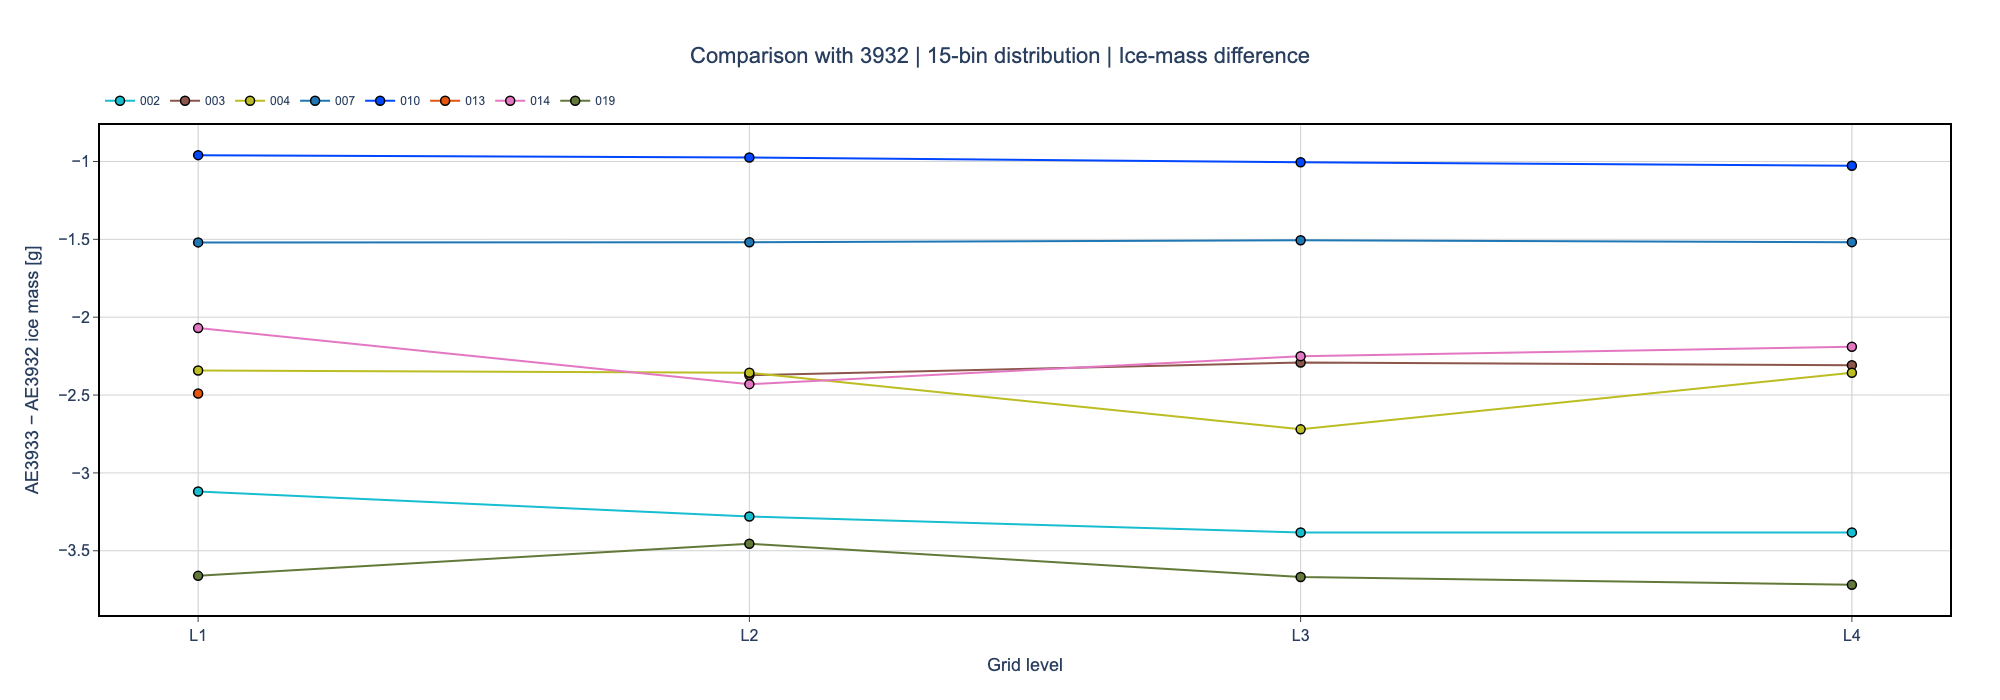
\includegraphics[width=\textwidth]{FIGURES/ICE_ACCRETION/tc_naca0012_ae3933_comparison_with_3932_ice_mass_bins15_difference.png}
\par}

\begin{block}{\scriptsize Assessment}
\begin{itemize}
    \item The matched-participant comparison directly isolates the ice-mass difference between AE3933 and AE3932.
    \item For most submissions, AE3933 predicts less ice mass than AE3932.
    \item The case-to-case difference remains comparatively consistent across the grid hierarchy for most submissions.
    \item This is the first clear systematic distinction between the two conditions after broadly comparable aerodynamic, impingement, and convective heat-transfer results.
\end{itemize}
\end{block}

\begin{alertblock}{\scriptsize Key Observation}
Despite comparable aerodynamic, impingement, and convective heat-transfer predictions, the two conditions begin to separate in the resulting ice mass. However, the approximately 15\% difference observed experimentally between the two conditions is not reproduced by the numerical predictions, which generally show a substantially smaller separation.
\end{alertblock}

\end{minipage}%
}

\end{frame}


% ============================================================
% ============================================================
% NACA0012 -- Ice Mass Droplet-Distribution Sensitivity
% ============================================================
% ============================================================

\begin{frame}{\small NACA0012 -- Ice Mass Sensitivity to Droplet Distribution}
\scriptsize

\begin{columns}[T,onlytextwidth]

\begin{column}{0.50\textwidth}
    \centering
    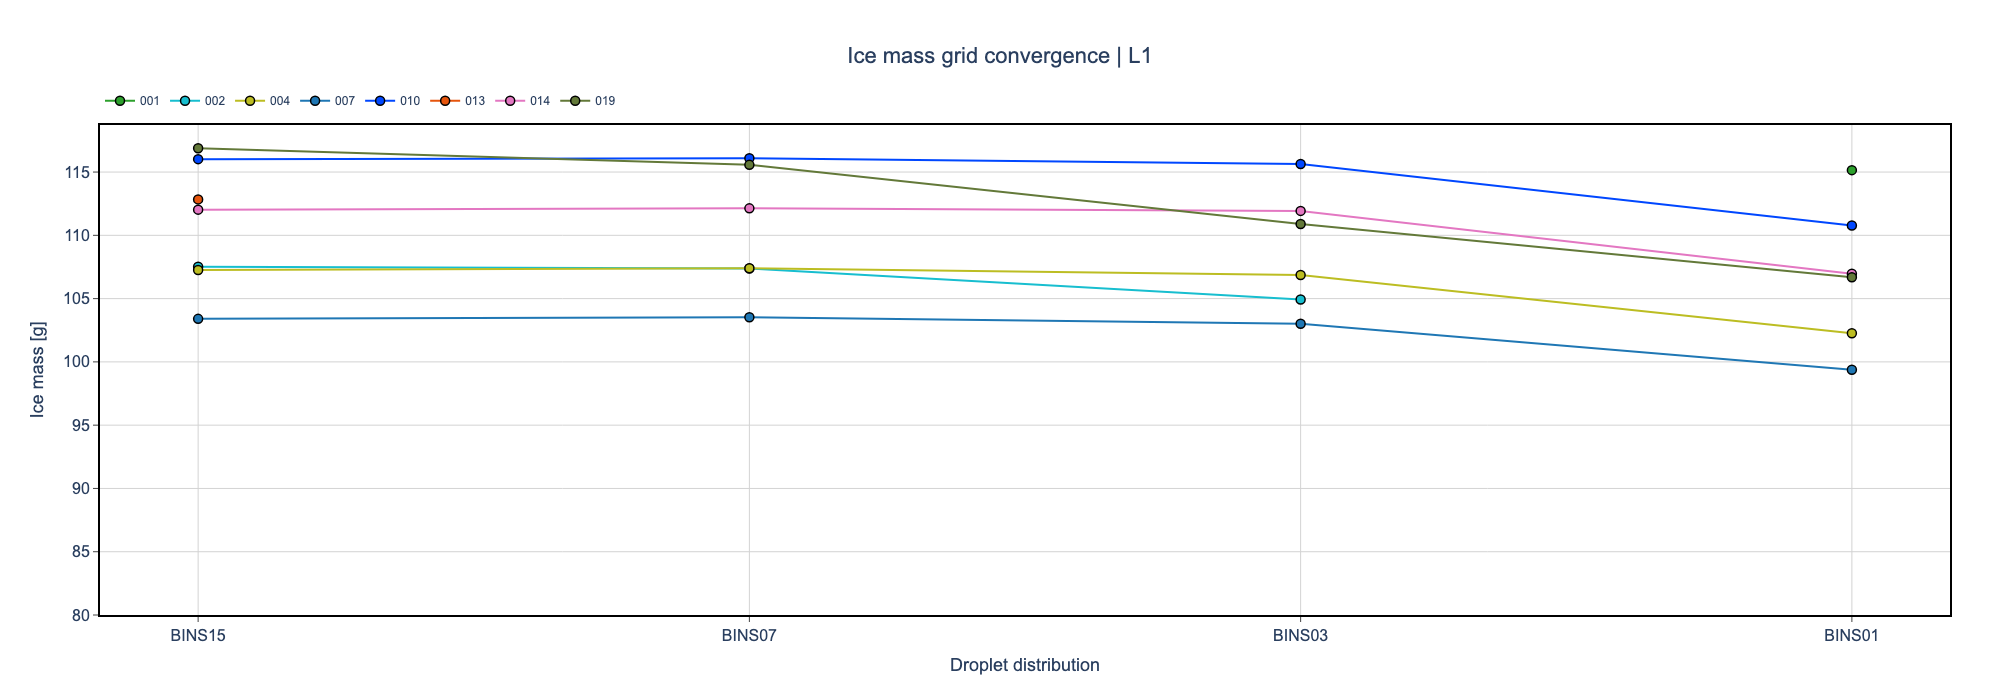
\includegraphics[width=\textwidth]{FIGURES/ICE_ACCRETION/tc_naca0012_ae3932_ice_mass_vs_n_unspecified_l1_vs_inverse_bins.png}

    \vspace{0.05cm}

    {\scriptsize\textbf{AE3932}}
\end{column}

\begin{column}{0.50\textwidth}
    \centering
    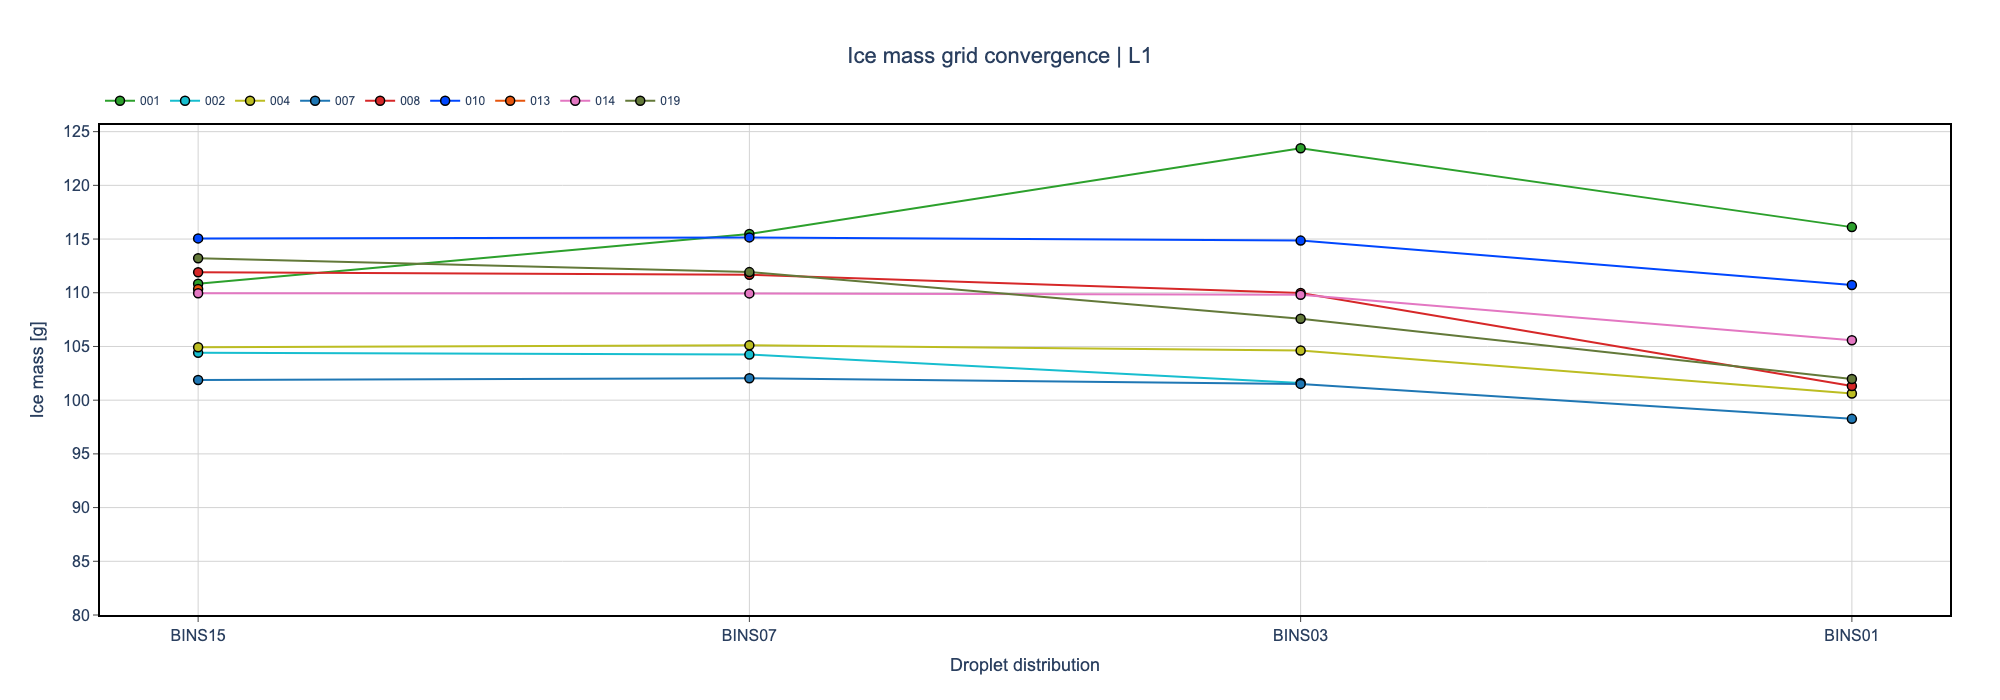
\includegraphics[width=\textwidth]{FIGURES/ICE_ACCRETION/tc_naca0012_ae3933_ice_mass_vs_n_unspecified_l1_vs_inverse_bins.png}

    \vspace{0.05cm}

    {\scriptsize\textbf{AE3933}}
\end{column}

\end{columns}

\vspace{0.15cm}

\begin{block}{\scriptsize Assessment}
\begin{itemize}
    \item The 15- and 7-bin distributions generally produce similar ice masses.
    \item Greater sensitivity appears as the droplet distribution is reduced to 3 and particularly 1 bin.
    \item For most submissions, reducing the droplet distribution modifies the ice mass more noticeably than the 15-to-7-bin reduction.
    \item The response is participant-dependent, indicating that droplet-size discretization influences the resulting icing response in addition to total water impingement.
\end{itemize}
\end{block}

\end{frame}


% ============================================================
% ============================================================
% NACA0012 -- Ice-to-Water Mass Ratio
% ============================================================
% ============================================================

\begin{frame}{\small NACA0012 -- Ice-to-Water Mass Ratio}
\scriptsize

\begin{columns}[T,onlytextwidth]

\begin{column}{0.50\textwidth}
    \centering
    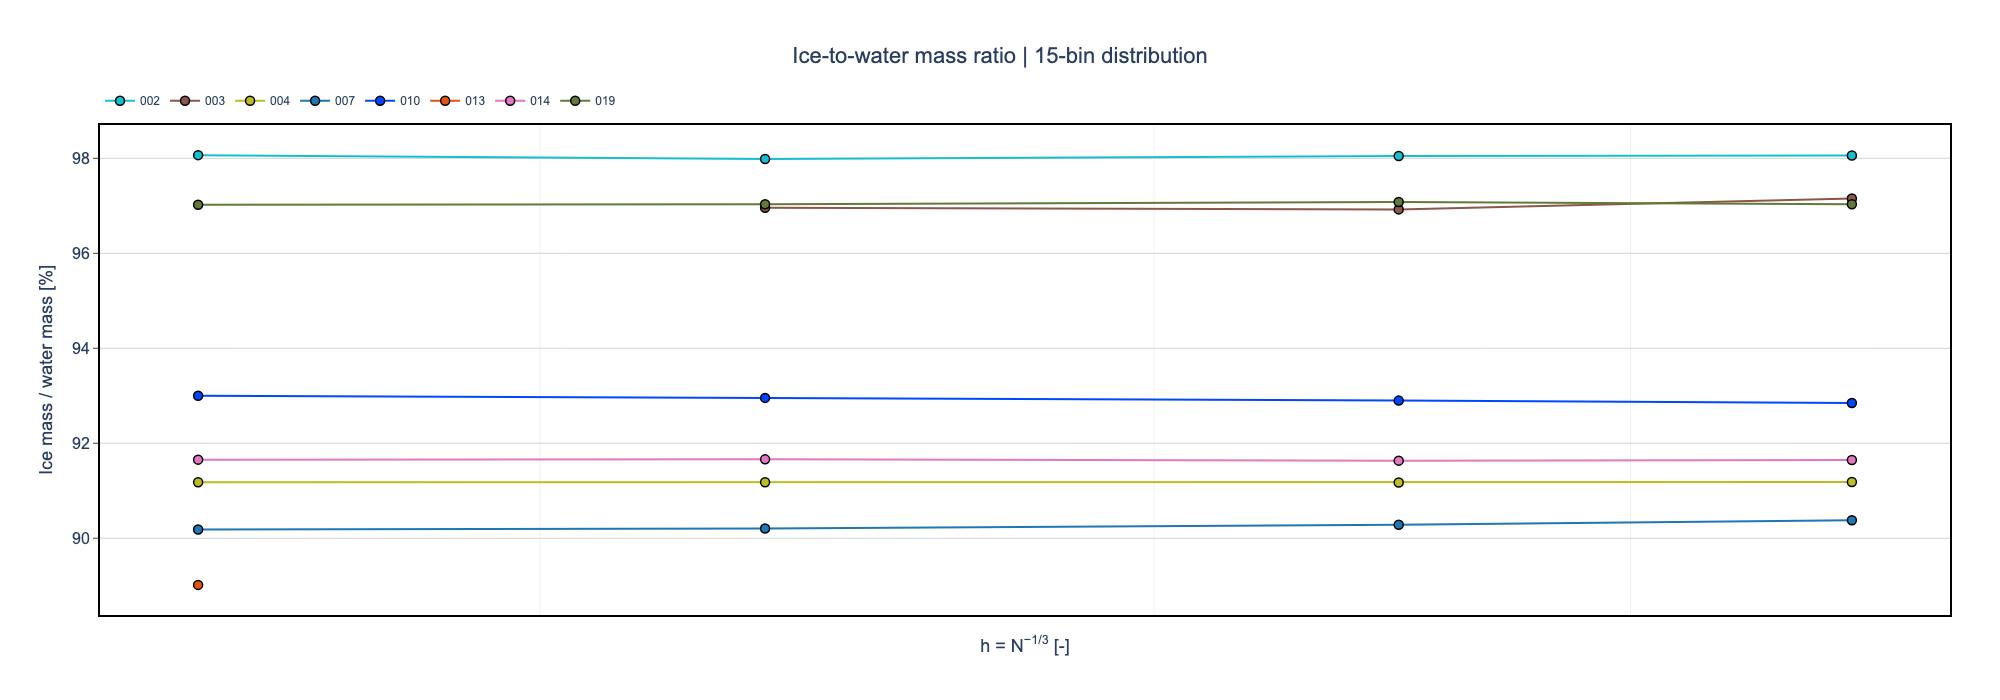
\includegraphics[width=\textwidth]{FIGURES/ICE_ACCRETION/tc_naca0012_ae3932_ice_to_water_ratio_vs_n_required_bins15.png}

    \vspace{0.05cm}

    {\scriptsize\textbf{AE3932}}
\end{column}

\begin{column}{0.50\textwidth}
    \centering
    \IfFileExists{FIGURES/ICE_ACCRETION/tc_naca0012_ae3933_ice_to_water_ratio_vs_n_required_bins15.png}{%
        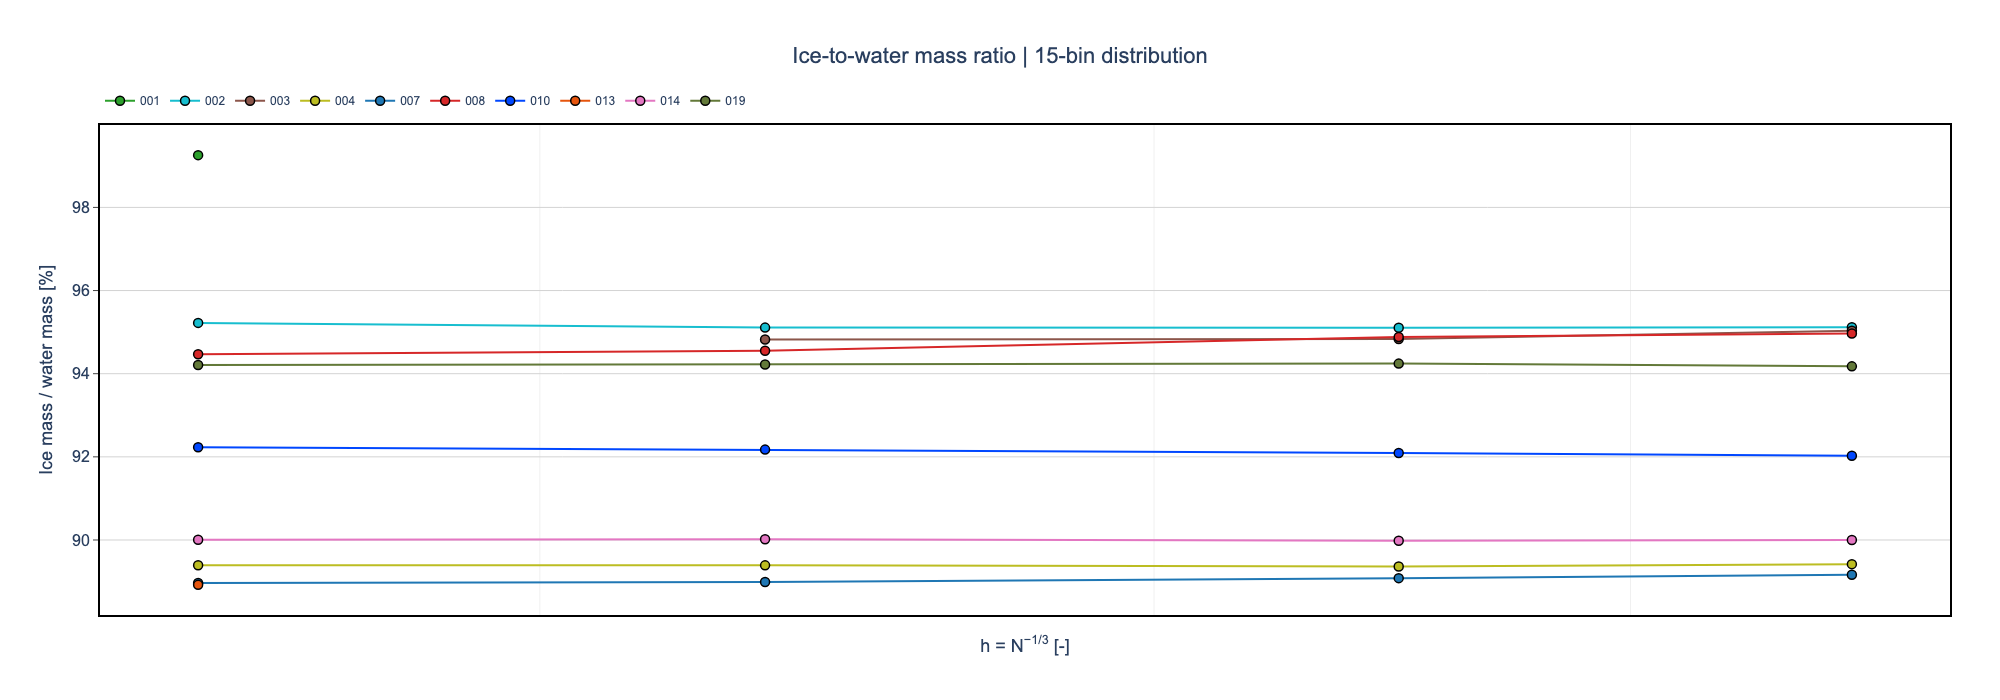
\includegraphics[width=\textwidth]{FIGURES/ICE_ACCRETION/tc_naca0012_ae3933_ice_to_water_ratio_vs_n_required_bins15.png}%
    }{%
        \fbox{\parbox[c][0.27\textheight][c]{0.92\textwidth}{\centering
        \scriptsize AE3933 ice-to-water ratio figure unavailable}}%
    }

    \vspace{0.05cm}

    {\scriptsize\textbf{AE3933}}
\end{column}

\end{columns}

\vspace{0.10cm}

\[
\frac{m_{\mathrm{ice}}}{m_{\mathrm{water}}}
\]

\vspace{0.05cm}

\begin{block}{\scriptsize Assessment}
\begin{itemize}
    \item Normalizing by the impinged water mass separates the icing response from differences in total water collection.
    \item Since the two conditions exhibit comparable water impingement, differences in this ratio directly highlight differences in the resulting ice accretion.
    \item The comparison therefore provides a clearer measure of the transition from impingement to the thermodynamic icing response.
\end{itemize}
\end{block}

\end{frame}


% ============================================================
% ============================================================
% NACA0012 -- Ice and Evaporation-to-Water Mass Ratio
% ============================================================
% ============================================================

\begin{frame}{\small NACA0012 -- Ice and Evaporation-to-Water Mass Ratio}
\scriptsize

\begin{columns}[T,onlytextwidth]

\begin{column}{0.50\textwidth}
    \centering
    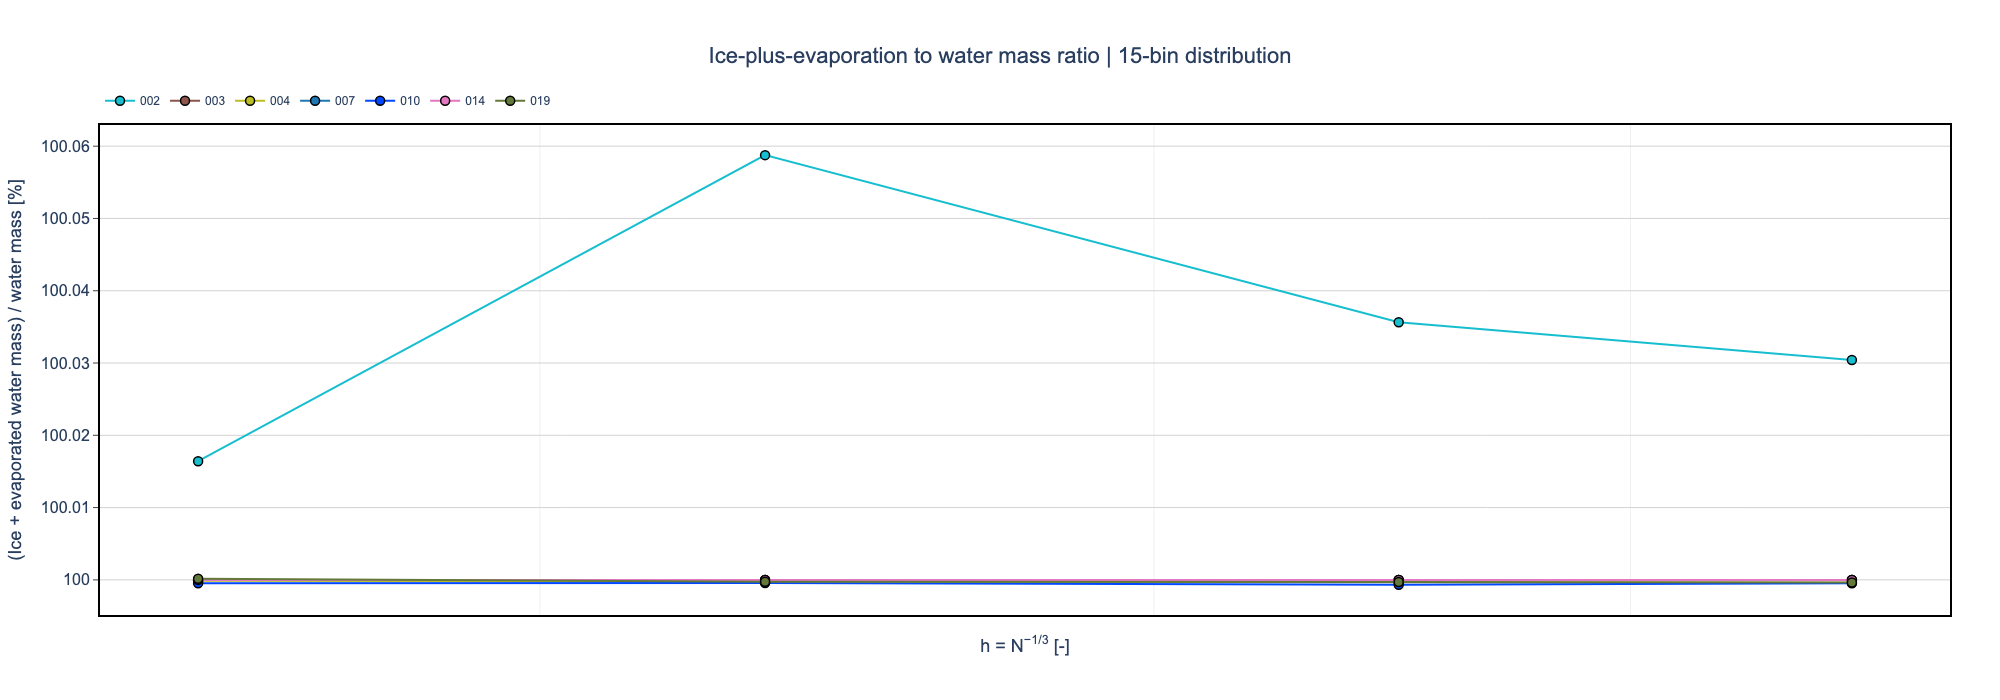
\includegraphics[width=\textwidth]{FIGURES/ICE_ACCRETION/tc_naca0012_ae3932_ice_evap_to_water_ratio_vs_n_required_bins15.png}

    \vspace{0.05cm}

    {\scriptsize\textbf{AE3932}}
\end{column}

\begin{column}{0.50\textwidth}
    \centering
    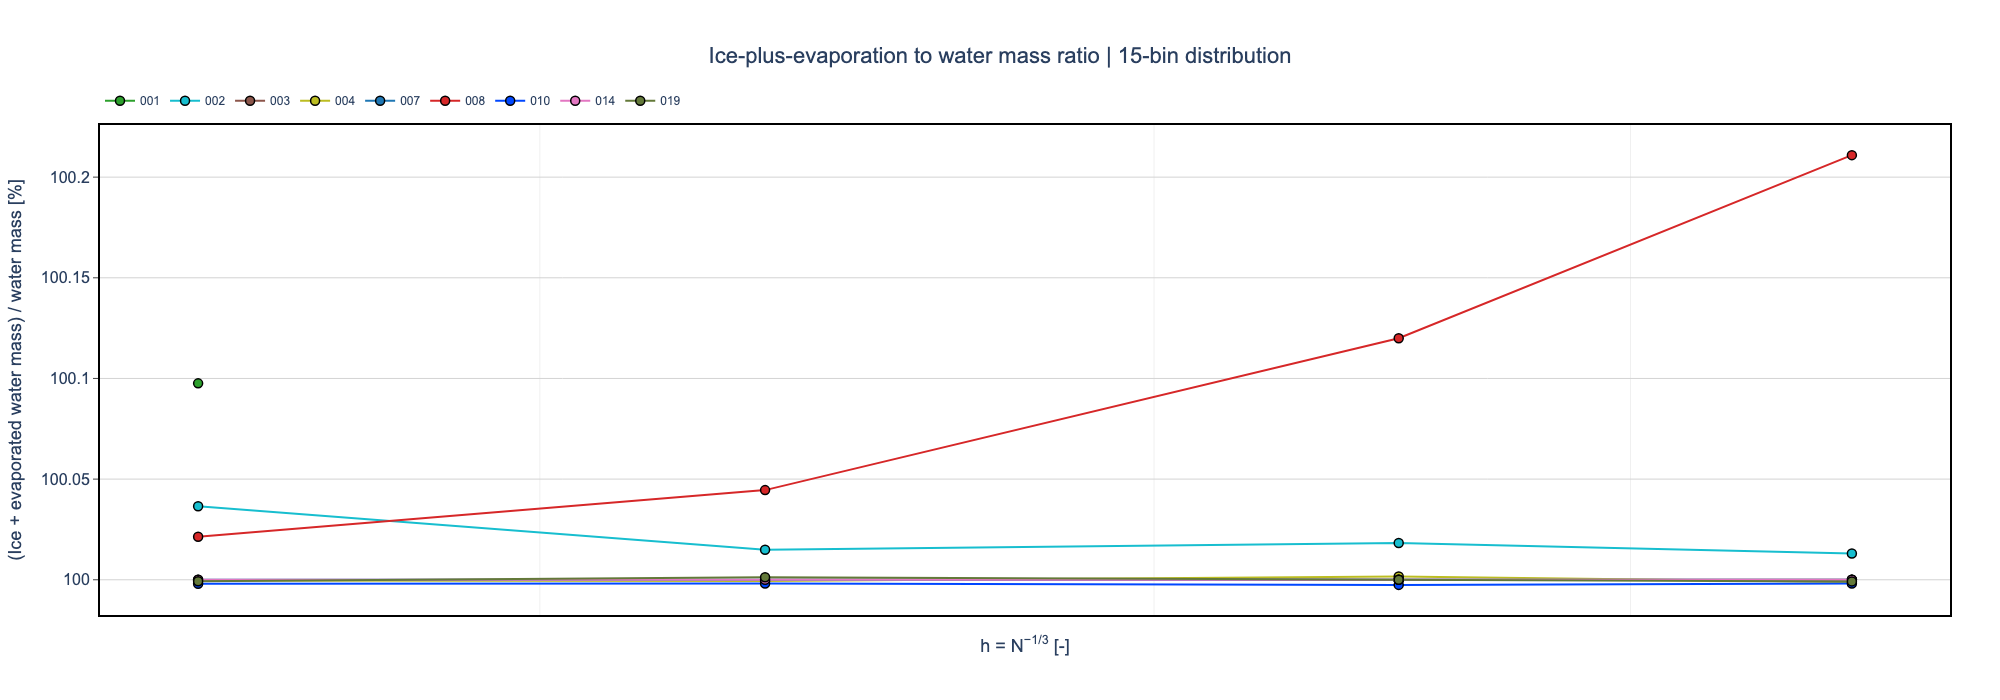
\includegraphics[width=\textwidth]{FIGURES/ICE_ACCRETION/tc_naca0012_ae3933_ice_evap_to_water_ratio_vs_n_required_bins15.png}

    \vspace{0.05cm}

    {\scriptsize\textbf{AE3933}}
\end{column}

\end{columns}

\vspace{0.10cm}

\[
\frac{m_{\mathrm{ice}}+m_{\mathrm{evap}}}{m_{\mathrm{water}}}
\]

\vspace{0.05cm}

\begin{block}{\scriptsize Assessment}
\begin{itemize}
    \item Including evaporated water provides additional information on the partition of the impinged water mass.
    \item Comparison with $m_{\mathrm{ice}}/m_{\mathrm{water}}$ identifies the contribution of evaporation to the difference between the two icing conditions.
    \item The remaining fraction represents water leaving the local ice-accretion balance through the other modeled mass-transfer mechanisms.
\end{itemize}
\end{block}

\end{frame}


% ============================================================
% ============================================================
% NACA0012 -- Upper Horn Angle Grid Convergence
% ============================================================
% ============================================================

\begin{frame}{\small NACA0012 -- Upper Horn Angle Grid Convergence}
\scriptsize

\begin{columns}[T,onlytextwidth]

\begin{column}{0.50\textwidth}
    \centering
    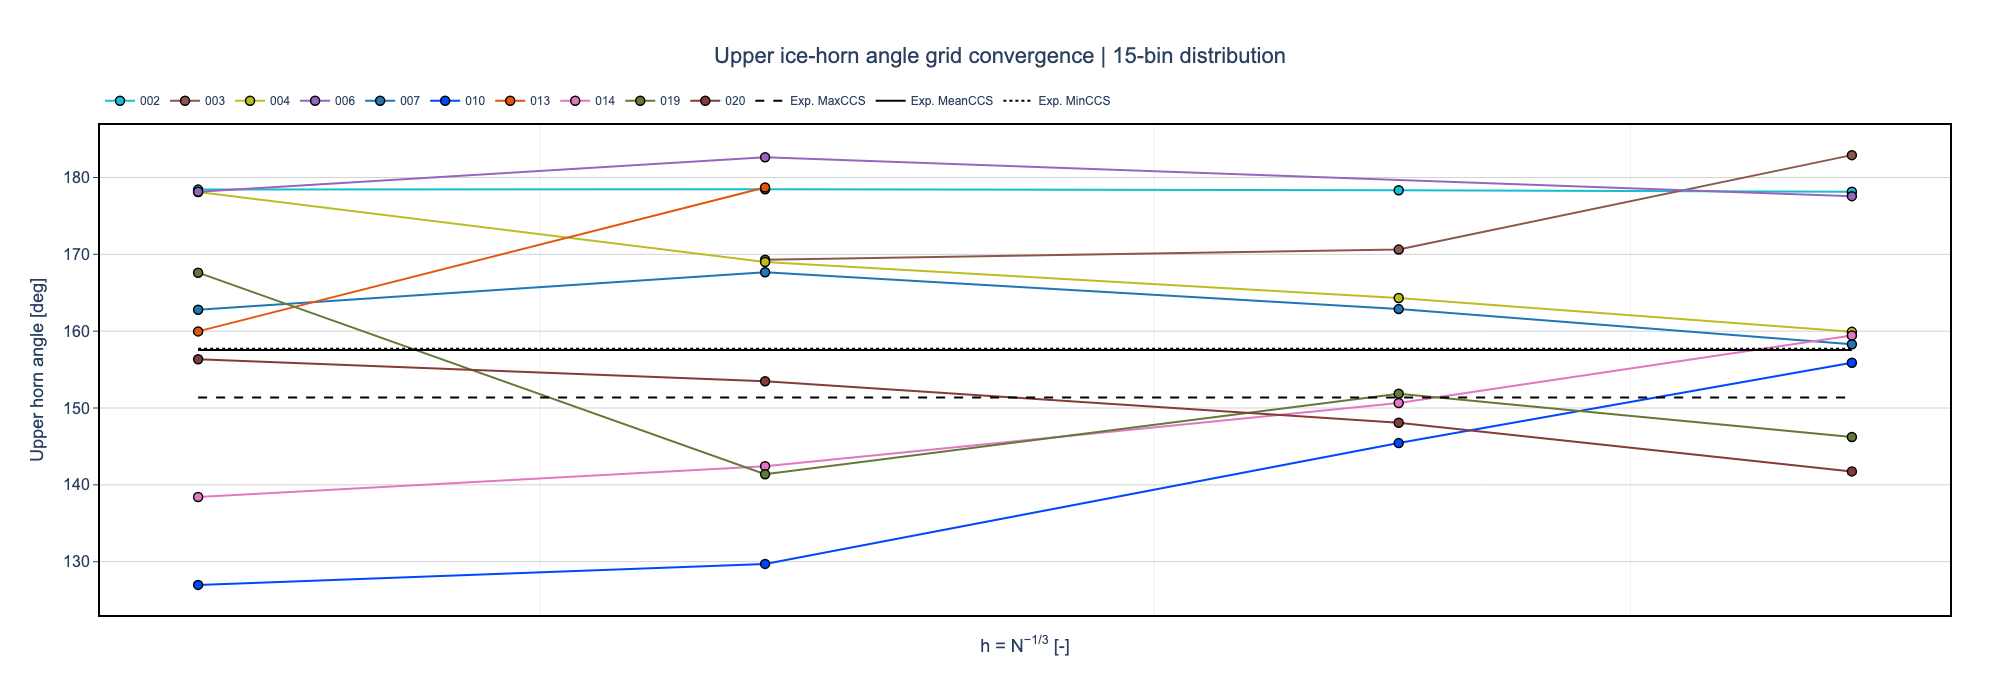
\includegraphics[width=\textwidth]{FIGURES/ICE_ACCRETION/tc_naca0012_ae3932_upper_horn_angle_bins15.png}

    \vspace{0.05cm}

    {\scriptsize\textbf{AE3932}}
\end{column}

\begin{column}{0.50\textwidth}
    \centering
    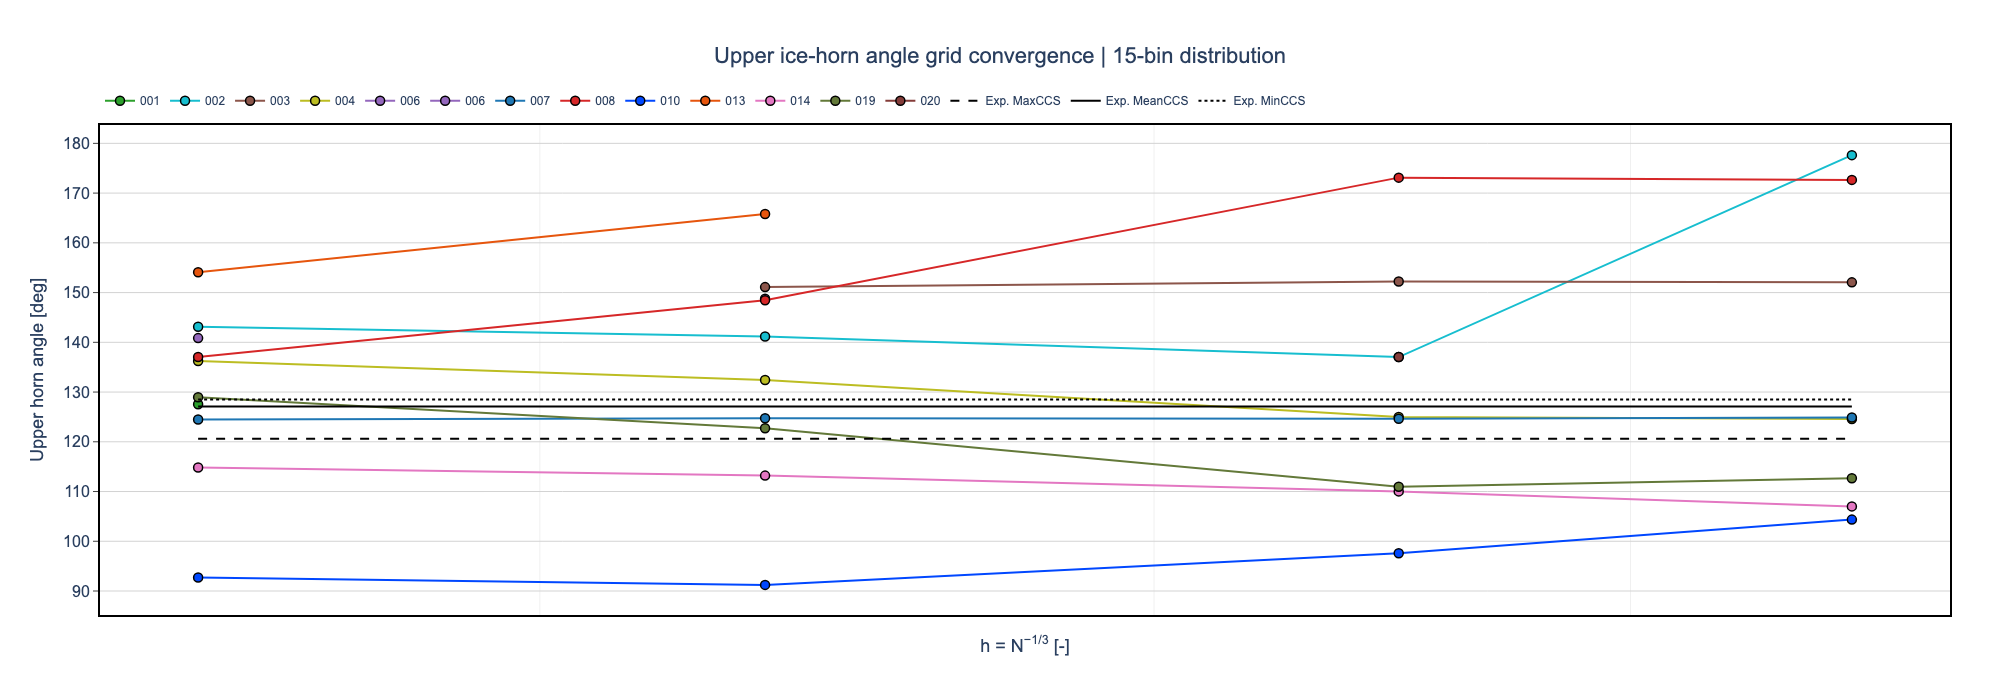
\includegraphics[width=\textwidth]{FIGURES/ICE_ACCRETION/tc_naca0012_ae3933_upper_horn_angle_bins15.png}

    \vspace{0.05cm}

    {\scriptsize\textbf{AE3933}}
\end{column}

\end{columns}

\vspace{0.15cm}

\begin{block}{\scriptsize Assessment}
\begin{itemize}
    \item The upper horn angle provides a geometric grid-convergence metric complementary to the integrated ice mass.
    \item Differences in horn orientation quantify changes in where the accreted ice is distributed rather than only how much ice is formed.
    \item Comparison between AE3932 and AE3933 indicates whether the change in icing response also produces a systematic change in horn orientation.
\end{itemize}
\end{block}

\end{frame}


% ============================================================
% ============================================================
% NACA0012 -- Upper Horn Angle Distribution Sensitivity
% ============================================================
% ============================================================

\begin{frame}{\small NACA0012 -- Upper Horn Angle Sensitivity to Droplet Distribution}
\scriptsize

\begin{columns}[T,onlytextwidth]

\begin{column}{0.50\textwidth}
    \centering
    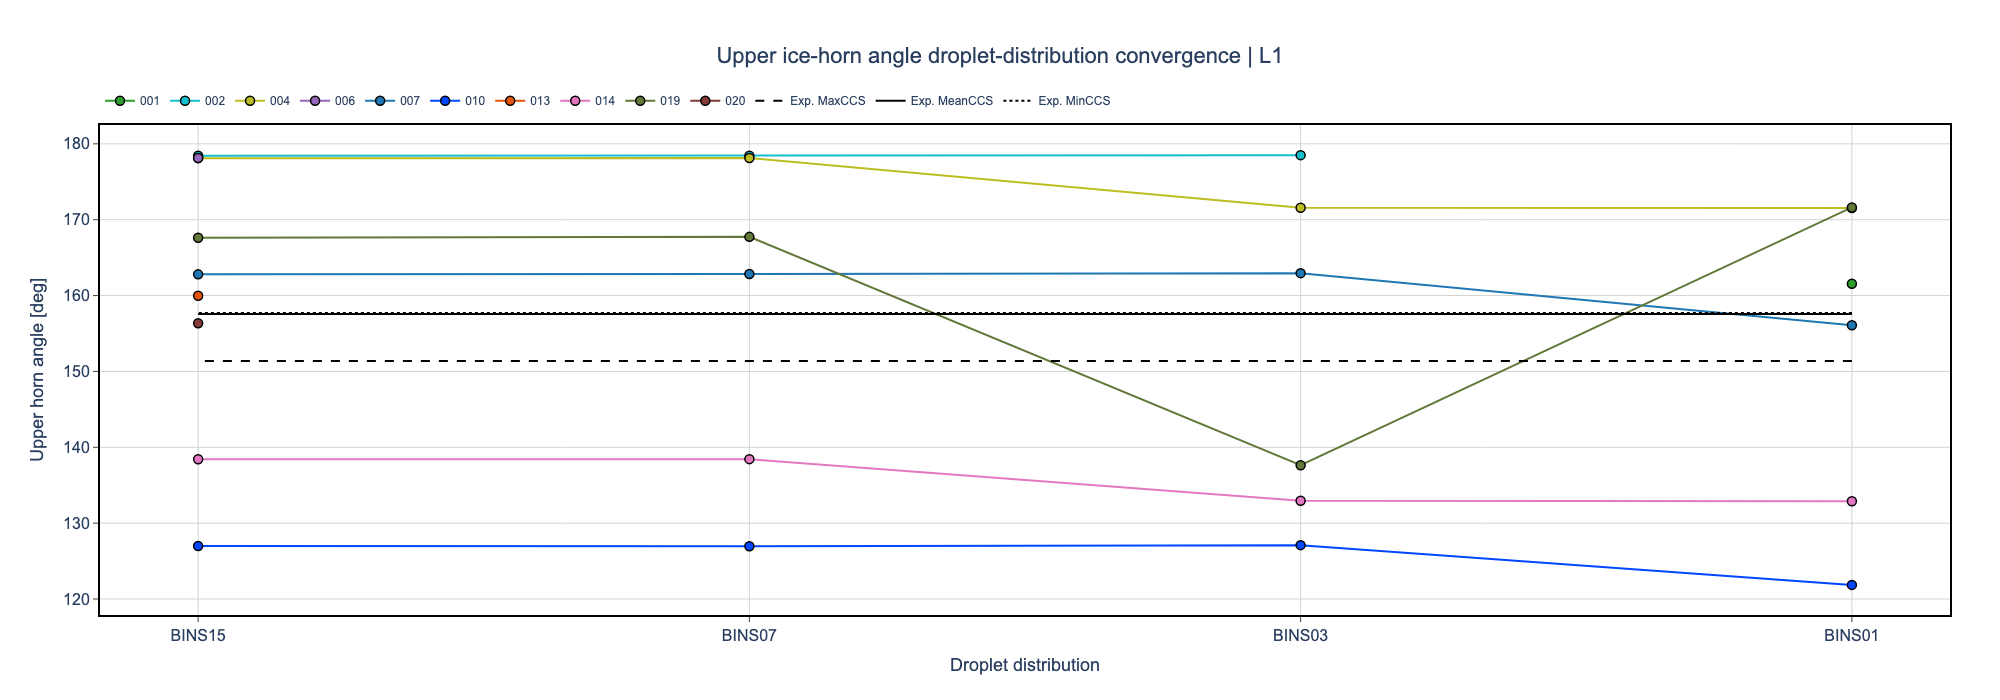
\includegraphics[width=\textwidth]{FIGURES/ICE_ACCRETION/tc_naca0012_ae3932_upper_horn_angle_distribution_convergence_l1.png}

    \vspace{0.05cm}

    {\scriptsize\textbf{AE3932}}
\end{column}

\begin{column}{0.50\textwidth}
    \centering
    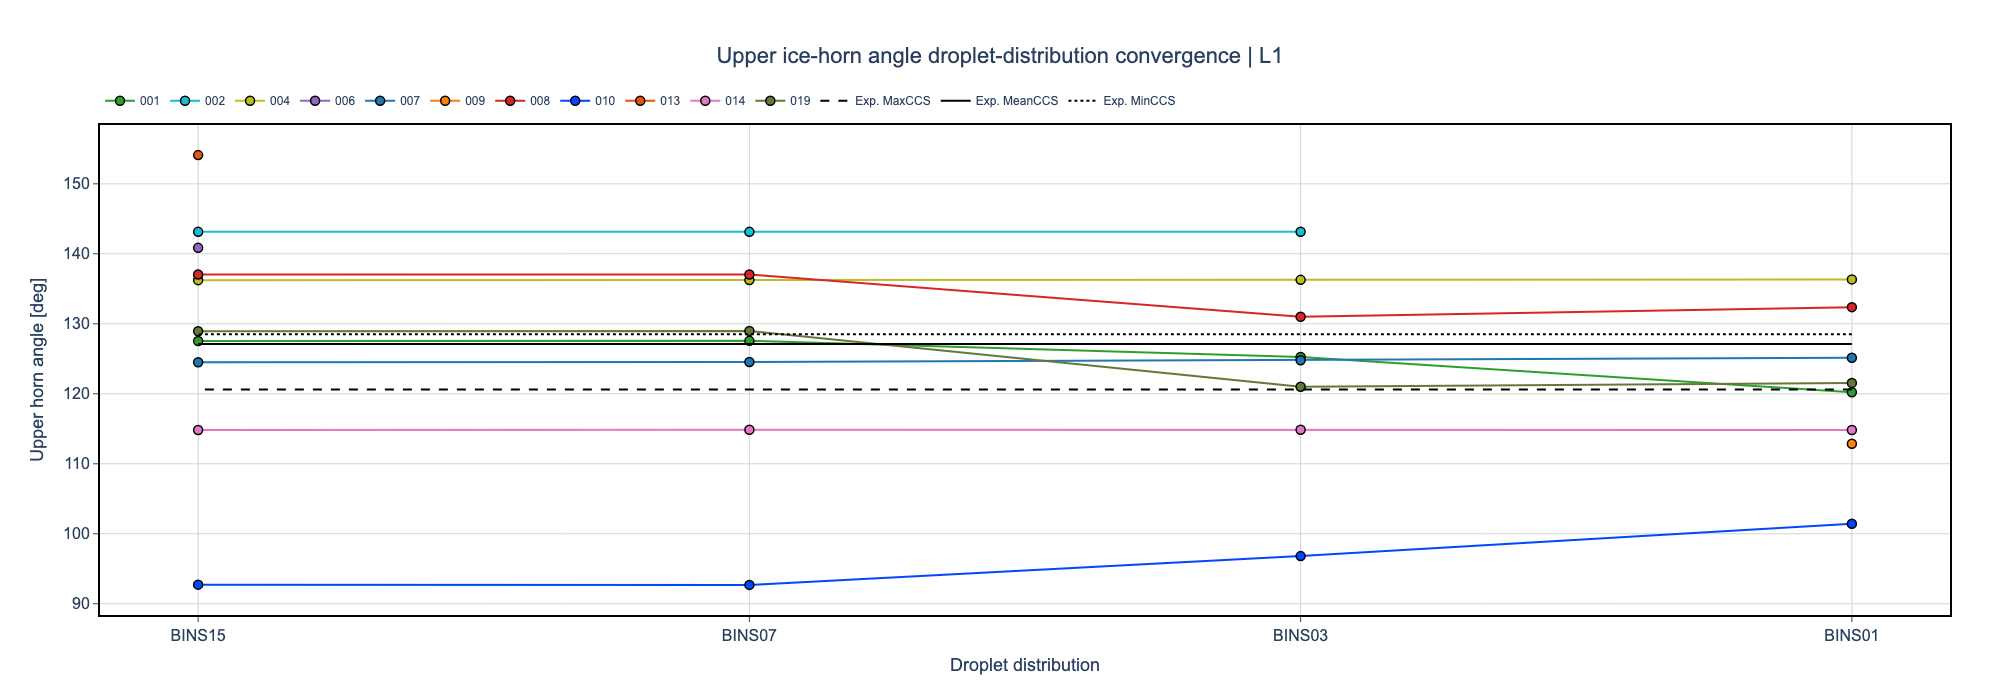
\includegraphics[width=\textwidth]{FIGURES/ICE_ACCRETION/tc_naca0012_ae3933_upper_horn_angle_distribution_convergence_l1.png}

    \vspace{0.05cm}

    {\scriptsize\textbf{AE3933}}
\end{column}

\end{columns}

\vspace{0.15cm}

\begin{block}{\scriptsize Assessment}
\begin{itemize}
    \item The L1 comparison evaluates the sensitivity of the upper horn orientation to droplet-size discretization.
    \item This provides a geometric counterpart to the ice-mass droplet-distribution sensitivity.
    \item Changes in total ice mass and changes in horn orientation should therefore be considered together when assessing droplet-distribution convergence.
\end{itemize}
\end{block}

\end{frame}


% ============================================================
% ============================================================
% NACA0012 -- Ice Shapes
% ============================================================
% ============================================================

\begin{frame}{\small NACA0012 -- Ice Shapes (L1, 15 Bins)}
\scriptsize

\begin{columns}[T,onlytextwidth]

\begin{column}{0.50\textwidth}
    \centering
    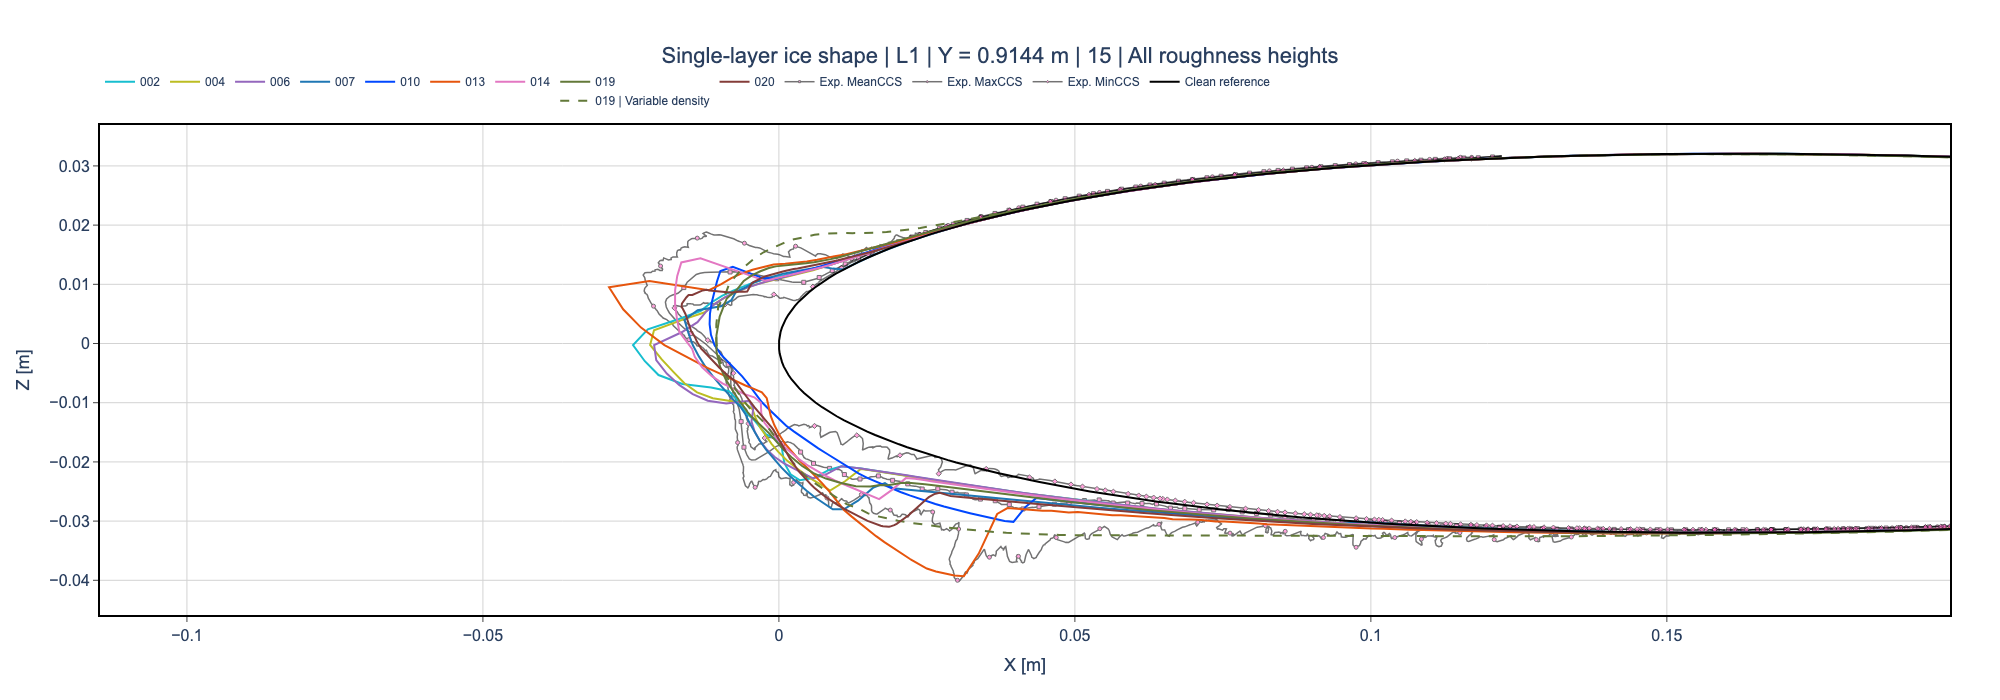
\includegraphics[width=\textwidth]{FIGURES/ICE_ACCRETION/tc_naca0012_ae3932_L1_single_layer_ice_shape_slice_0p9144_bins15_roughness_unspecified.png}

    \vspace{0.05cm}

    {\scriptsize\textbf{AE3932}}
\end{column}

\begin{column}{0.50\textwidth}
    \centering
    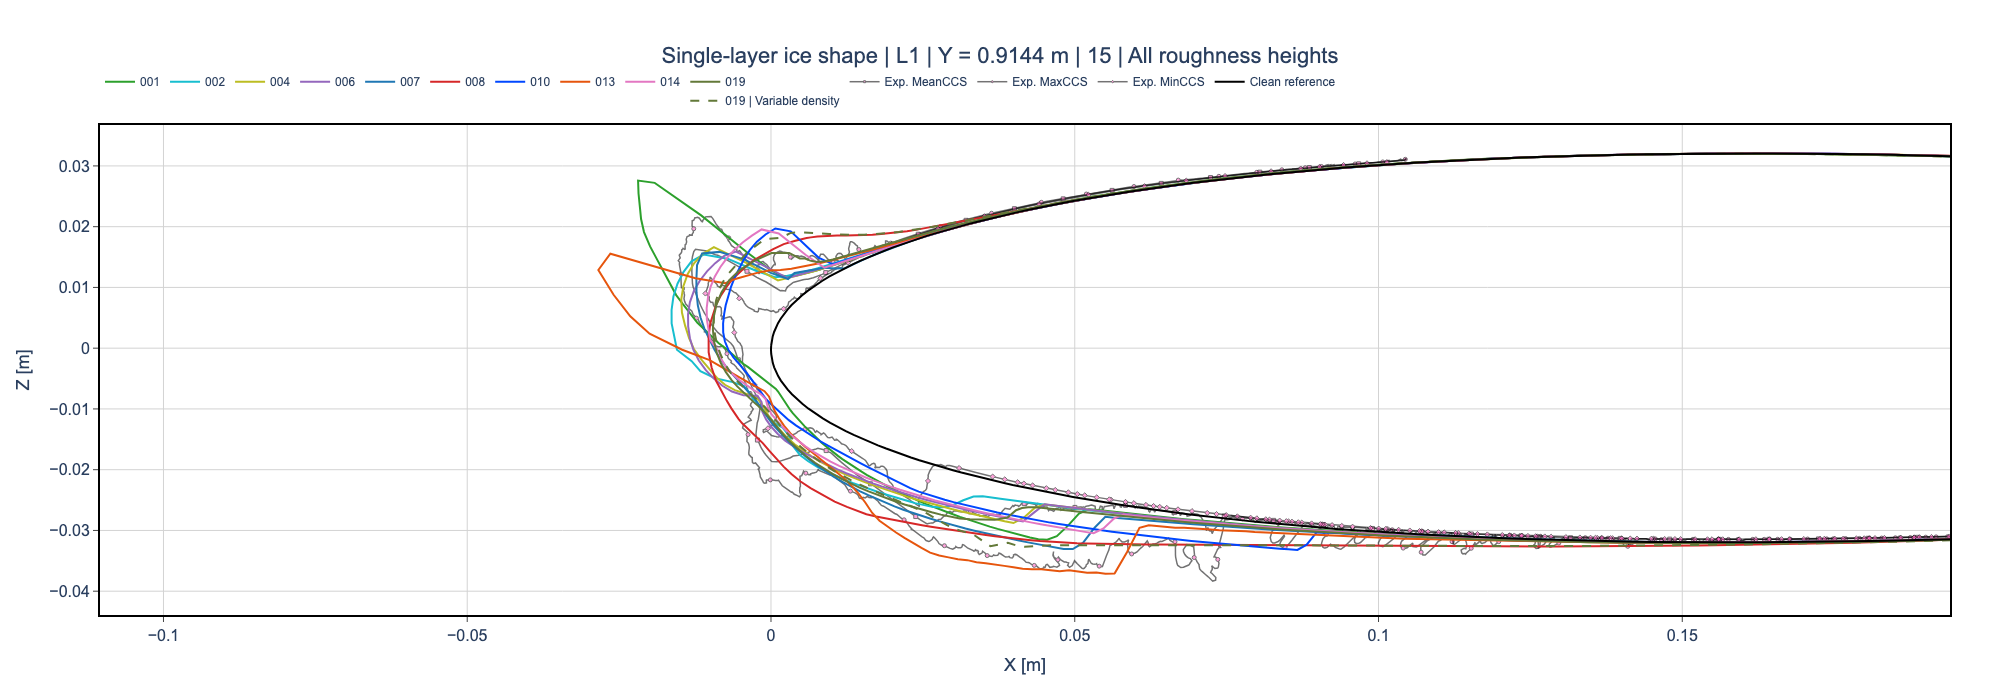
\includegraphics[width=\textwidth]{FIGURES/ICE_ACCRETION/tc_naca0012_ae3933_L1_single_layer_ice_shape_slice_0p9144_bins15_roughness_unspecified.png}

    \vspace{0.05cm}

    {\scriptsize\textbf{AE3933}}
\end{column}

\end{columns}

\vspace{0.15cm}

\begin{block}{\scriptsize Assessment}
\begin{itemize}
    \item The L1 15-bin ice shapes provide the final geometric comparison of the two icing conditions.
    \item The comparison reveals how differences in ice mass and mass partition translate into horn orientation, local thickness, and overall accretion extent.
    \item Experimental ice shapes provide the validation reference for the predicted spatial accretion pattern.
\end{itemize}
\end{block}

\end{frame}


% ============================================================
% ============================================================
% NACA0012 -- Ice Accretion Summary
% ============================================================
% ============================================================

\begin{frame}[shrink]{\small NACA0012 -- Ice Accretion Summary}
\scriptsize

\begin{block}{\scriptsize Ice Mass}
\begin{itemize}
    \item Most submissions exhibit limited 15-bin ice-mass sensitivity to spatial grid refinement, with isolated stronger grid dependence.
    \item In contrast to the preceding quantities, a systematic difference begins to emerge between AE3932 and AE3933 in the resulting ice mass.
\end{itemize}
\end{block}

\vspace{0.15cm}

\begin{block}{\scriptsize Mass Partition}
\begin{itemize}
    \item The ice-to-water mass ratio separates the icing response from the comparable water impingement between the two conditions.
    \item Including evaporation further identifies how the impinged water is partitioned between ice formation and other mass-transfer mechanisms.
\end{itemize}
\end{block}

\vspace{0.15cm}

\begin{block}{\scriptsize Ice Geometry}
\begin{itemize}
    \item Horn-angle metrics complement the integrated mass quantities by quantifying the spatial distribution of the accreted ice.
    \item The L1 15-bin ice shapes provide the final geometric comparison with the experimental accretions.
\end{itemize}
\end{block}

\vspace{0.15cm}

\begin{alertblock}{\scriptsize Ice Accretion Takeaway}
Aerodynamic, impingement, and convective heat-transfer quantities remain broadly comparable between AE3932 and AE3933, while the icing response begins to distinguish the two conditions. The mass-partition and geometric metrics show how this difference propagates from total ice mass to the final ice shape.
\end{alertblock}

\end{frame}


% ============================================================
% ============================================================
% END -- NACA0012 ICE ACCRETION
% ============================================================
% ============================================================
